\documentclass{article}
\usepackage[margin=1.5cm,bottom=2cm]{geometry}
\usepackage{fancyhdr}
\usepackage{graphicx}
\usepackage[section]{placeins}
\pagestyle{fancy}
\usepackage{hyperref}
\usepackage[export]{adjustbox}
\pagestyle{fancy}
\usepackage{xcolor}
\hypersetup{colorlinks=true,urlcolor=blue,urlbordercolor=blue}
\begin{document}
\fancyhead[L]{ 
\includegraphics[width=2cm]{au_logo.png} }
\fancyhead[R]{ENGR 2310: Computational Problem Solving}
\fancyfoot[C]{\thepage}
\vspace*{0cm}
\begin{center}
	{\LARGE \textbf{Homework 2}}\\
	\vspace{.25cm}
	{\Large Projectile Motion}
	%\vspace{0.25cm}
	%{\Large Due: Friday, September 4}
\end{center}

Write a program which prompts the user to supply the initial speed (in m/s) and initial height above landing point (in meters) of a launched projectile. Your program will find the launch angle $\theta$ (in degrees) which maximizes the \textit{range} (the horizontal distance traveled) of the projectile.

\begin{figure}[ht!]
	\centering
	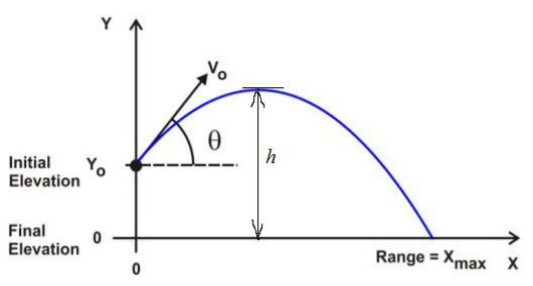
\includegraphics[width=10cm]{image.png}
\end{figure}

Assuming the projectile's trajectory is only affected by gravity then we know the time of flight $\Delta t$ (the time taken for the ball to land):

\begin{equation}
\Delta t=\frac{v_i\sin{\theta}+\sqrt{v_i^2\sin^2{\theta}+2g y_i }}{g}
\label{tof}
\end{equation}
Where $v_i$ is the initial speed, $y_i$ is the initial height, and $g=9.81$ m$\cdot$s$^{-2}$ is the acceleration due to gravity at the surface of the Earth. 

The horizontal distance traveled is then:
\begin{equation}
x_\mathrm{max}=v_i\cos{\theta}\Delta t
\end{equation}

Given $v_i$ and $y_i$, your program should calculate (to within $0.1^\circ$) which angle (between 0 and 90$^\circ$) maximizes $x_\mathrm{max}$.
\textit{Hint: one way to do this is to calculate $x_\mathrm{max}$ for every value of $\theta$ between 0 and 90, in steps of 0.1, and then pick the angle that corresponds to the largest $x_\mathrm{max}$}

\subsection*{Requirements}
Your program should utilize (at least) two functions (not including \texttt{main()}):
\begin{enumerate}
	\item A function \texttt{time\_of\_flight(theta,vi,yi)} which uses the angle, initial velocity, and initial height to calculate and return $\Delta t$
	\item A function \texttt{xrange(theta,vi,yi)} which first makes a call to \texttt{time\_of\_flight(theta,vi,yi)}, and then returns the quantity $v_i\cos{\theta}\Delta t$
\end{enumerate}
Your program should follow the style and readability guidelines detailed \href{https://drive.google.com/file/d/1SFf6Rhv8LydlrUhf85QhMuiZb_IKRS4N/view?usp=sharing}{here}
\end{document}